\section{Umsetzung in TwinCAT}	\label{Umsetzung_Prozessmodell}
	\subsection{Allgemeine Struktur} \label{Prozessmodell_Allgemeine Struktur}
	
		Innerhalb der Umsetzung wurden zwei verschiedenen Strukturen erarbeitet und getestet. 
		
		\textbf{Struktur 1:} Skills instanziiert in separatem Programm
		\vspace{2mm} 
		\vspace{-5mm} 
		\\
		\begin{wrapfigure}{r}{0.5\textwidth}
			\centering
			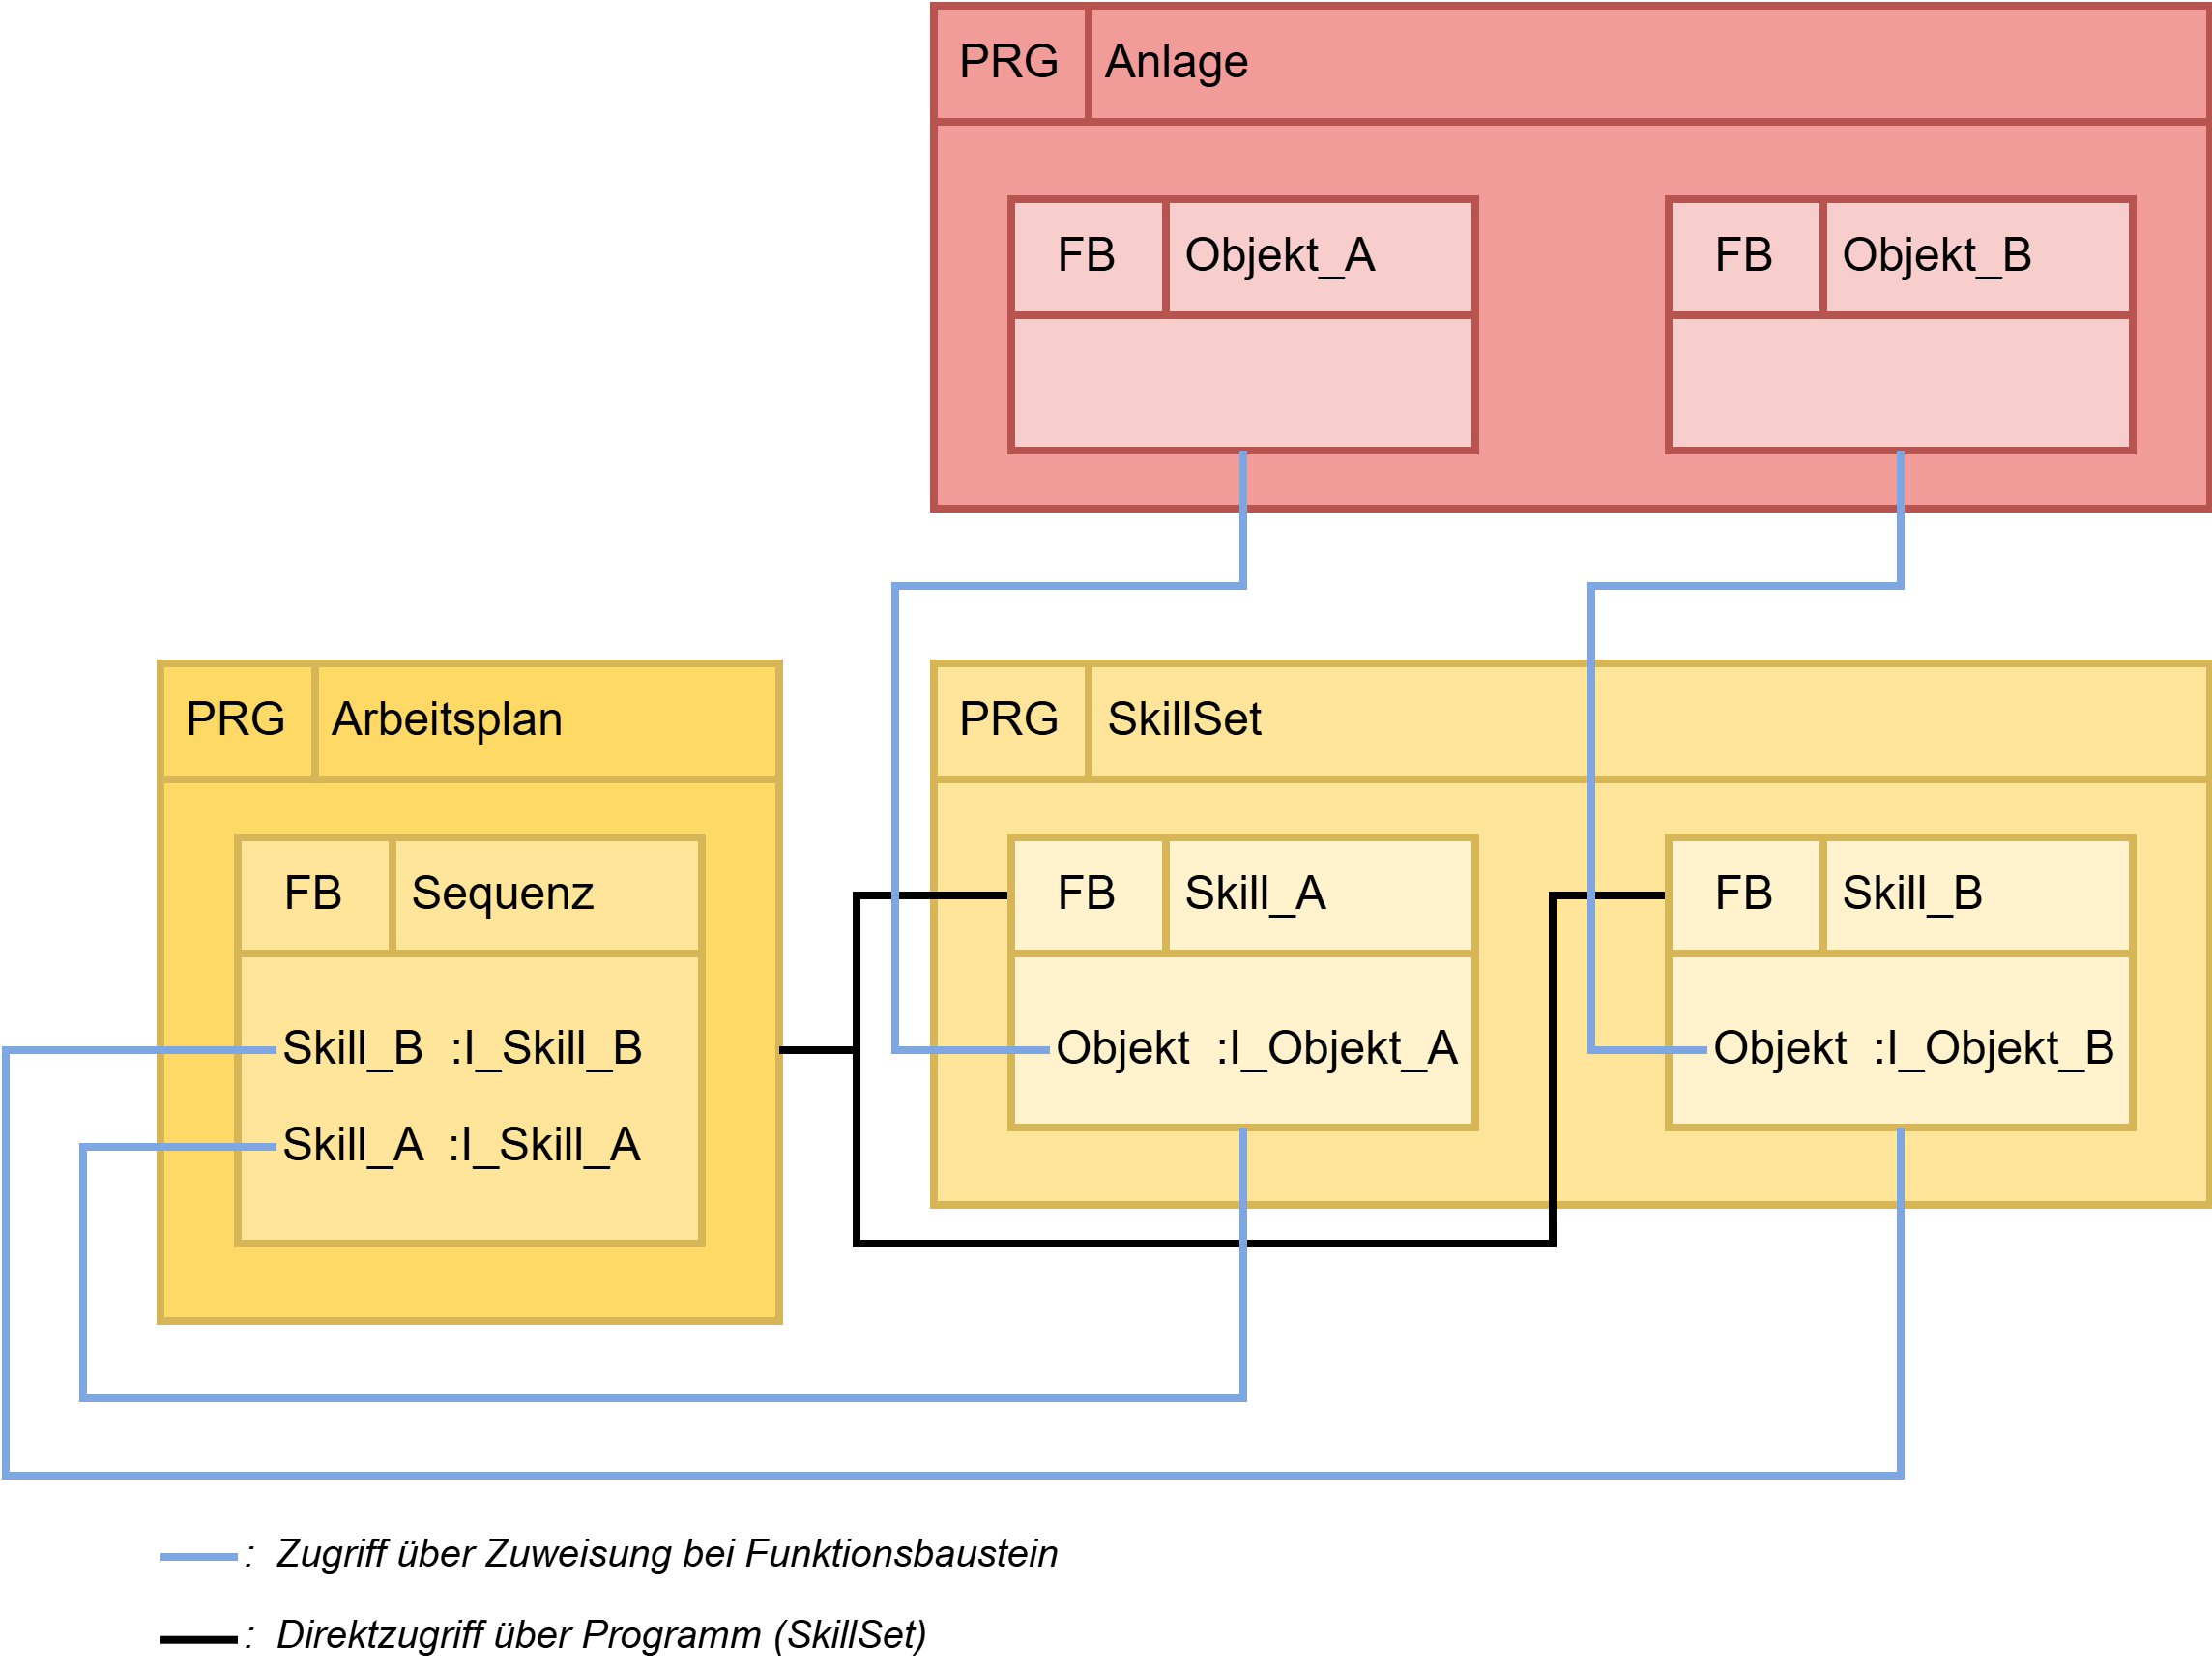
\includegraphics[width=0.45\textwidth]{08_Prozessmodell/Struktur_1}
			\captionsetup{justification=centering}
			\caption{Prozessmodell-Struktur 1}
			\label{fig:Prozessmodell_Struktur_1}
		\end{wrapfigure}
		In der ersten Struktur wurden die Skills in einem Programm namens «SkillSet» instanziiert, vergleichbar mit den Objekten innerhalb der Anlage. Diese instanziierten Skills können anschliessend vom Arbeitsplan oder über Sequenzen verwendet werden. Der Arbeitsplan greift dabei direkt auf die im SkillSet-Programm instanziierten Skills zu. Sequenzen hingegen erhalten die Skills über Eingangsvariablen, die mit dem entsprechenden Interface definiert wurden.
		\\
		Der Vorteil dieser Struktur liegt darin, dass die Skills kontinuierlich ausgeführt werden, wodurch jederzeit der aktuelle Zustand eines Skills festgestellt werden kann. Die Interaktion mit den Skills wird durch diese Struktur einfacher und transparenter (Probleme bei der Interaktion werden im Zusammenhang mit der zweiten Struktur genauer beschrieben).
		\\
		Ein Nachteil dieser Struktur besteht darin, dass alle benötigten Skills vorab im SkillSet-Programm instanziiert werden müssen. Beispielsweise: Wenn ein Roboter 10 Skills besitzt und das System um einen zweiten Roboter erweitert wird, müssen auch für diesen zweiten Roboter die 10 entsprechenden Skills im SkillSet-Programm instanziiert werden. Dadurch entsteht eine gewisse Abhängigkeit des Prozessmodells vom Anlagenmodell.
		\\
		Ein weiteres Risiko ist die mögliche Verwechslung von Skills, insbesondere bei zwei gleichartigen Skills für unterschiedliche Komponenten. Wenn beispielsweise Roboter A angesprochen werden soll, könnte versehentlich der Skill von Roboter B ausgewählt werden.
	
		\textbf{Struktur 2:} Instanziierung von Skills innerhalb von Arbeitsplänen und Sequenzen
		\vspace{2mm} 
		\vspace{-5mm}
		\\
		\begin{wrapfigure}{r}{0.4\textwidth}
			\centering
			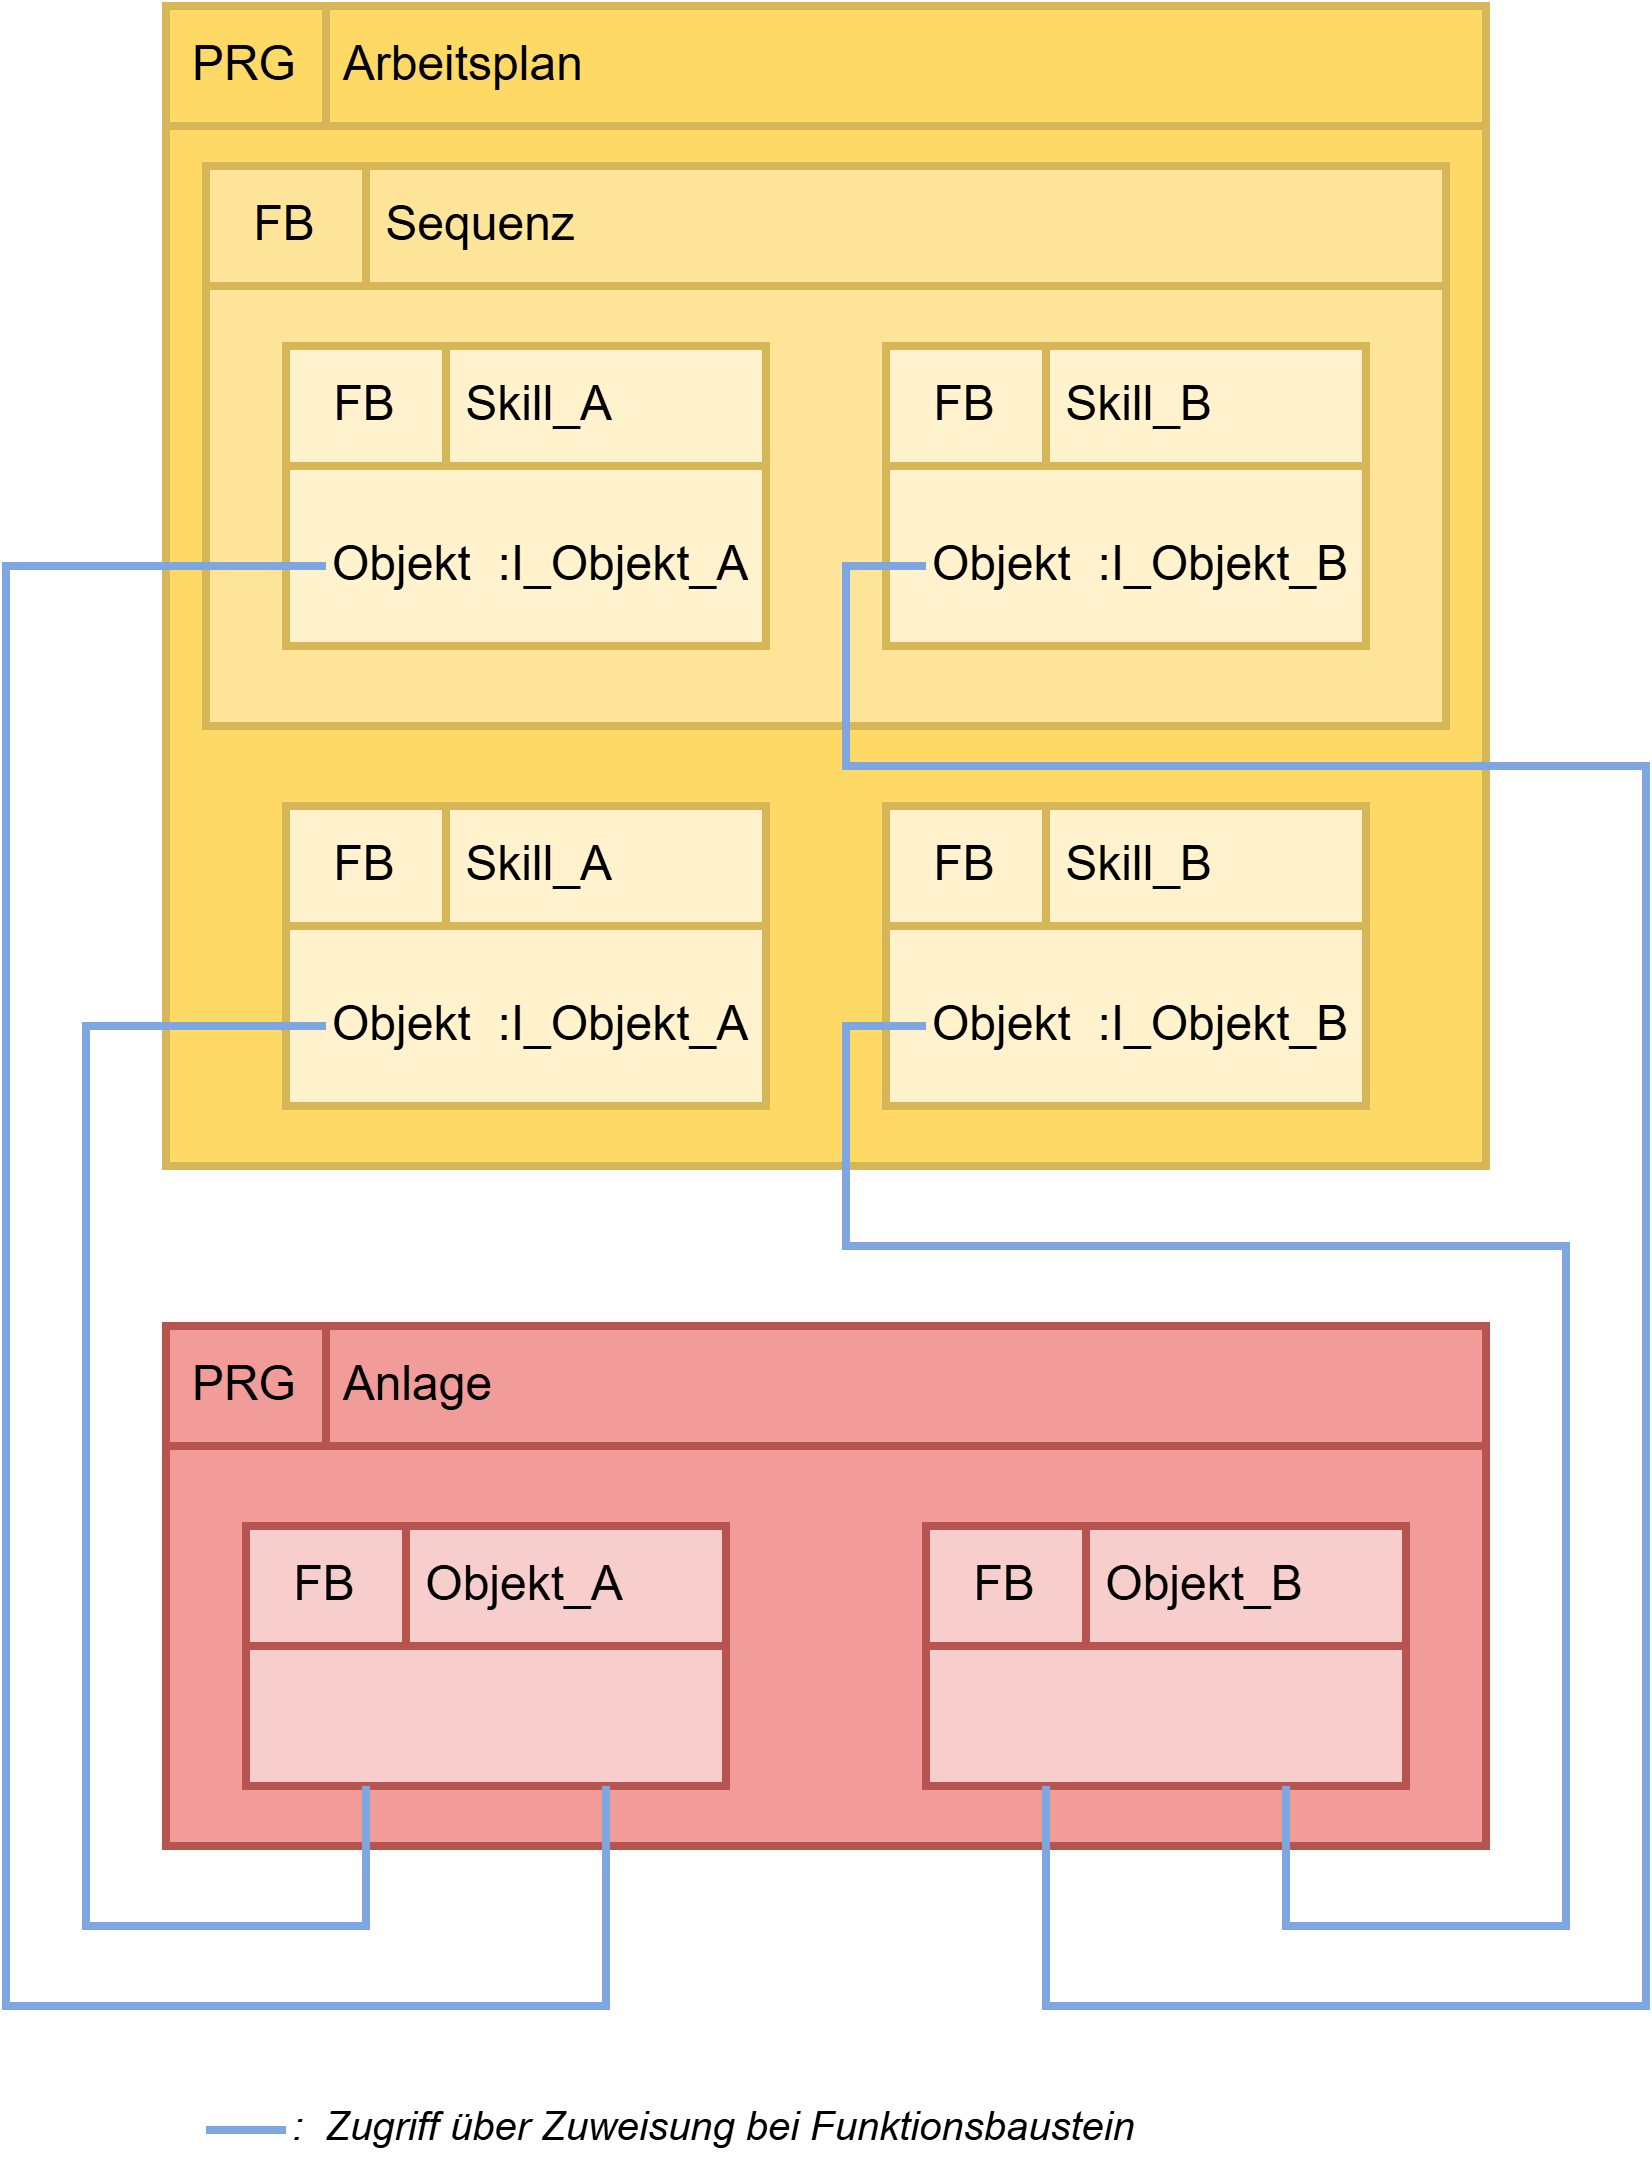
\includegraphics[width=0.35\textwidth]{08_Prozessmodell/Struktur_2}
			\captionsetup{justification=centering}
			\caption{Prozessmodell-Struktur 2}
			\label{fig:Prozessmodell_Struktur_2}
		\end{wrapfigure} 
		Bei dieser Struktur werden ausschliesslich die Skills innerhalb des Arbeitsplans oder der Sequenz instanziiert, die tatsächlich benötigt werden. Auch die Zuweisung der Objekte erfolgt direkt innerhalb des Arbeitsplans oder der Sequenz. Eine Interface-Implementierung der Skills ist hierbei nicht erforderlich. Der entsprechende Skill wird innerhalb eines Schritts aufgerufen, alle notwendigen Parameter (z.B. das Objekt) werden zugewiesen, und der Skill wird ausgeführt.
		\\
		Ein wesentlicher Vorteil der Struktur besteht darin, dass die Skills lokal in dem jeweiligen Arbeitsplan oder der Sequenz instanziiert werden. Ebenso erfolgt die Zuweisung der Objekte lokal, wodurch das Prozessmodell keine Informationen über das Anlagenmodell benötigt, wie etwa die Anzahl der im System vorhandenen Roboter. Stattdessen wird der benötigte Roboter einfach dem entsprechenden Skill innerhalb des Arbeitsplans oder der Sequenz zugewiesen. Diese Herangehensweise verbessert zudem die Übersichtlichkeit und Verständlichkeit der Software: Durch die instanziierten Skills lässt sich schnell erkennen, welche Aufgaben eine bestimmte Sequenz oder ein Arbeitsplan ausführt.
		\\
		Ein Nachteil dieser Struktur ist jedoch, dass beim Aufruf, der Zuweisung und der Ausführung der Skills potenziell mehr Probleme auftreten können. Es ist essenziell, ein Verständnis darüber zu haben, wie lange Informationen für die Verarbeitung benötigen und wie auf Methoden zugegriffen werden kann. Diese Struktur erfordert daher ein fundiertes Wissen über TwinCAT und dessen Funktionsweise.
		
	\subsection{Aufbau einer Sequenz} \label{Prozessmodell_Sequenzaufbau}
		Der Schwerpunkt liegt dabei, den allgemeinen Aufbau einer Sequenz zu erklären. Es werden nicht alle definierten Sequenzen aufgezeigt und beschrieben. Die Sequenzen unterscheiden sich grundsätzlich nur in den definierten Ablaufschritten und den verwendeten Skills. Zusätzlich konnten zum Zeitpunkt dieser Dokumentation konnten noch nicht alle Sequenzen komplett abgeschlossen werden. 
		\\
		Eine Sequenz basiert auf einem Funktionsbaustein, der in strukturiertem Text (\Gls{ST}) erstellt ist. Der Funktionsbaustein umfasst verschiedene Aktionen. Eine Aktion ist für den Ablauf verantwortlich, der als \Gls{SFC} umgesetzt wird. Die übrigen Aktionen bestehen aus Zuweisungen, die ebenfalls in strukturiertem Text geschrieben sind. Diese dienen innerhalb des Ablaufs dazu, Skills aufzurufen und Parameter an diese zu übergeben. Über den Funktionsbausteine «\verb|FB_Basis|» werden der Sequenz die Steuerungselemente vererbt. 
		\\
		\begin{figure}[H]
			\centering
			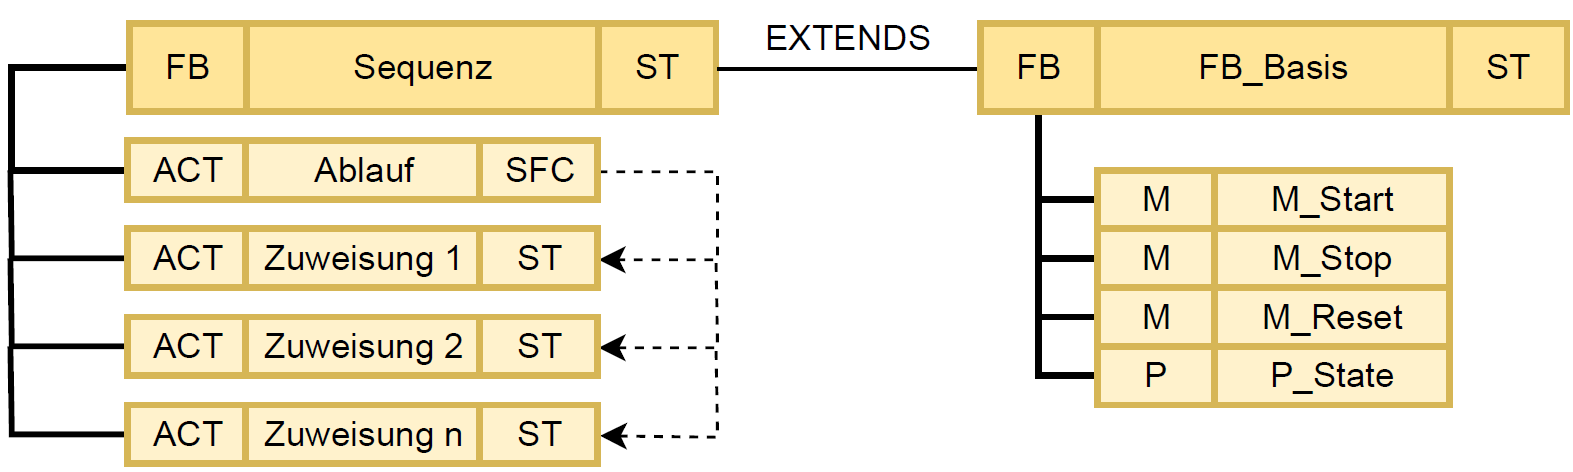
\includegraphics[width=1\textwidth]{08_Prozessmodell/Sequenzaufbau}
			\captionsetup{justification=centering}
			\caption{Aufbau einer Sequenz}
			\label{fig:Sequenzaufbau}
		\end{figure}
		
		Als Beispiel wird die Sequenz «\verb|Seq_Teile_Hohlen|» betrachtet. Die Aufgabe diese Frequenz ist es, mit dem Roboter an eine definierte Position zu fahren und ein Teil mit dem Greifer zu packen. 
		
		\newpage
		
		Der Funktionsbaustein wurde dabei wie folgt  definiert: 
		
		\begin{figure}[h!]
			\centering
			\begin{subfigure}[b]{0.58\textwidth}
				\centering
				\fbox{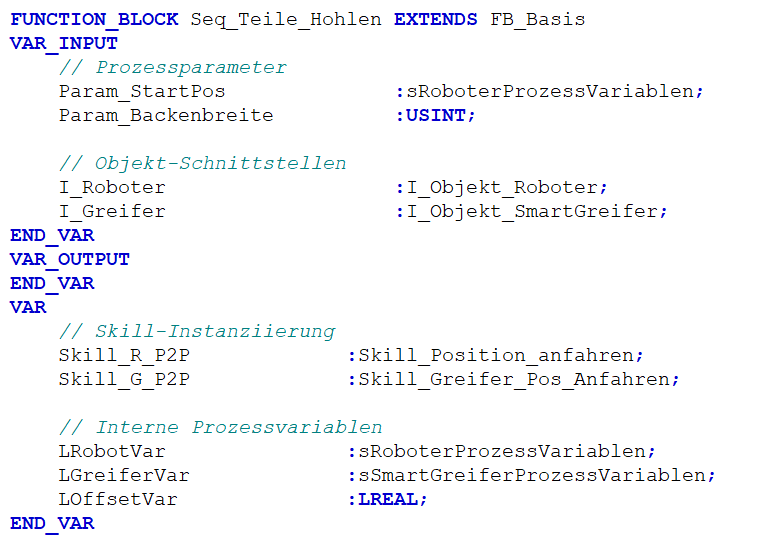
\includegraphics[width=\textwidth]{08_Prozessmodell/Sequenz_FB_1}}
				\caption{Variablendeklaration}
				\label{fig:Sequent_Variablendeklaration}
			\end{subfigure}
			\hfill
			\begin{subfigure}[b]{0.30\textwidth}
				\centering
				\fbox{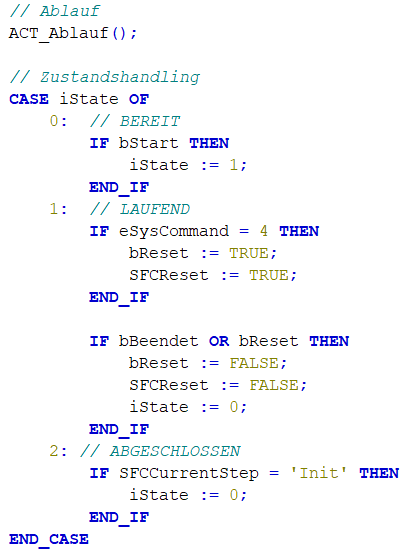
\includegraphics[width=\textwidth]{08_Prozessmodell/Sequenz_FB_2}}
				\caption{Funktionsbausteinprogrammierung}
				\label{fig:Sequenz_Funktionsbausteinprogrammierung}
			\end{subfigure}
			\caption{Sequenz-Funktionsbaustein}
			\label{fig:SequenzFunktionsbaustein}
		\end{figure} 
		
		Für die Funktionalität des Bausteins müssen zwei Prozessparameter sowie Objekte als Eingabevariablen definiert werden. Die Prozessparameter legen die Startposition und die Greifer-Backenbreite im geöffneten Zustand fest. Die erforderlichen Objekte umfassen den Roboter und den Greifer, die jeweils über das entsprechende Interface instanziiert werden.
		Innerhalb der internen Variablen werden sowohl die benötigten Skills als auch Variablen zur Zuweisung der Prozessparameter initialisiert.
		\\
		Im Baustein selbst wird zunächst der Ablauf «\verb|ACT_Ablauf|» ausgeführt. Diese Aktion läuft kontinuierlich. Das Zustandshandling erfolgt durch eine CASE-Struktur, die den aktuellen Zustand verarbeitet und die entsprechenden Aktionen steuert.
		\\
		\\
		Die Aktion «\verb|ACT_Ablauf|» ist wie folgt definiert: 
		\\
		\begin{figure}[H]
			\centering
			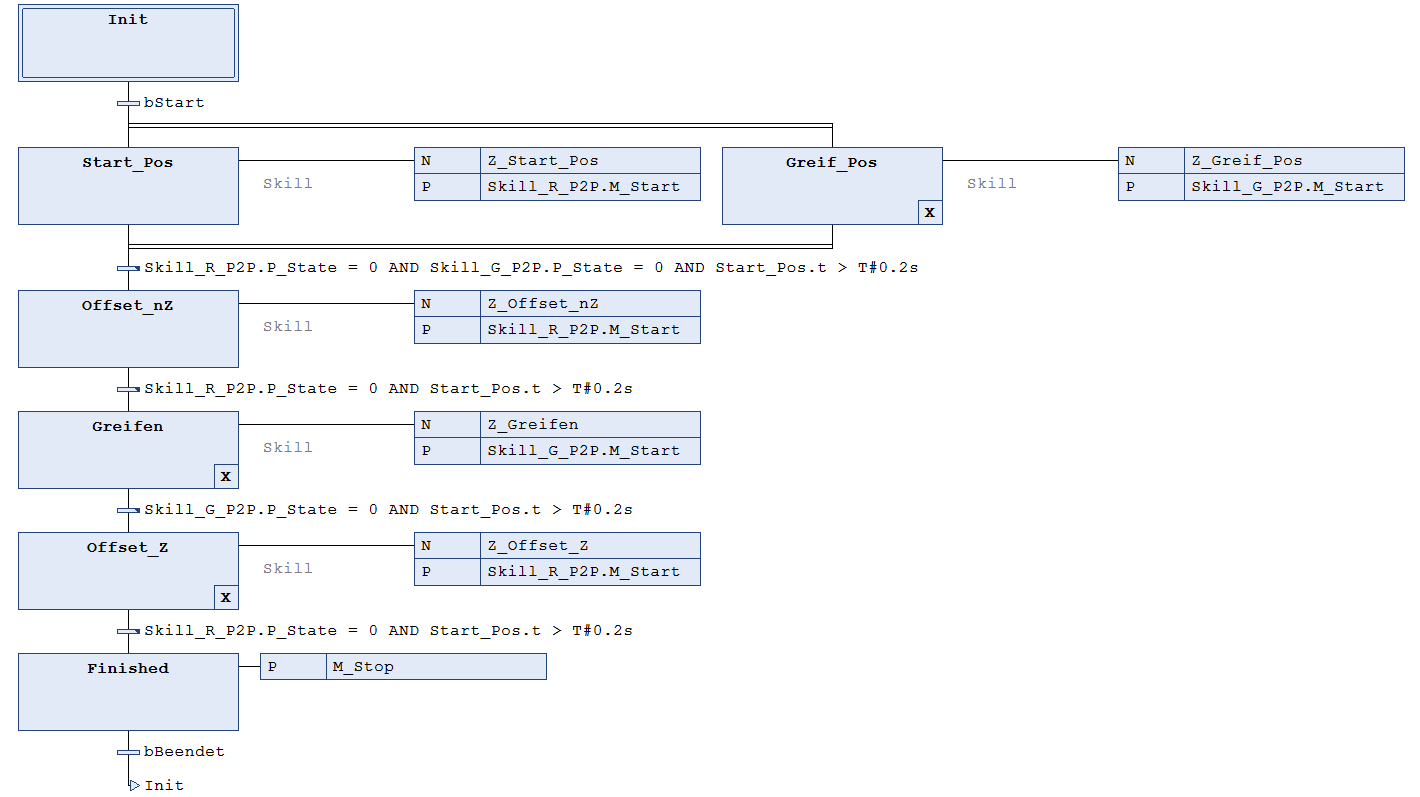
\includegraphics[width=1\textwidth]{08_Prozessmodell/ACT_Ablauf}
			\captionsetup{justification=centering}
			\caption{Beispiel für Sequenzablauf}
			\label{fig:Sequenzablauf}
		\end{figure}
		
		\newpage
		
		Zu Beginn wird der Roboter und Greifer in eine definierte Startposition gebracht. Von dieser Position fährt der Roboter nach unten und greift nach dem Teil. Als letzter Schritt bewegt sich der Roboter mit dem Teil nach oben. Ein grundsätzlich sehr einfacher und überschaubarer Ablauf. Mit der Variablen Startposition für Roboter und  Greifer, kann diese Sequenz für alle Elemente der Anwendung so übernommen werden.
		\\
		Jeder Schritt ruft zwei Aktionen auf.  Innerhalb der ersten Aktion wird der Skill aufgerufen und die Parameter werden zugewiesen. Diese Aktion wird kontinuierlich durchgeführt, solange der Schritt aktiv ist. 
		\\
		\begin{figure}[H]
			\centering
			\fbox{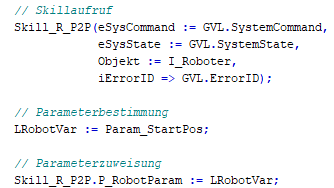
\includegraphics[width=.5\textwidth]{08_Prozessmodell/Sequenz_Aktion_Zuweisung}}
			\captionsetup{justification=centering}
			\caption{Zuweisungsaktion der Sequenz}
			\label{fig:Sequenz_Zuweisung}
		\end{figure}
		
		Die zweite Aktion führt die die Methoden zum Starten des Skills aus. Im Moment werden die Start-Methoden mit dem \Gls{SFC}-Qualifizierer «P» umgesetzt.  Das «P» steht dabei für «Pulse». In TwinCAT bedeutet dies, dass die Methode zwei Mal durchgeführt wird: Einmal, wenn der Schritt aktiv wird und ein zweites Mal im darauffolgenden Zyklus. Dieses Verhalten hat zu Problemen geführt. Zusätzlich kann mit dem Qualifizierer «P» auch nicht innerhalb eines \Gls{SFC}-Ablaufs zwei Mal, in separaten Schritten, auf eine Methode zugegriffen werden. Aus im Moment unbekannten Gründen, ist die Methode nach dem ersten Schritt gesperrt. 
		\vspace{2mm} 
		\\
		Es stehen zwei mögliche Herangehensweisen zur Verfügung:
		\vspace{2mm} 
		\\
		\textbf{Möglichkeit 1: } Tiefergehende Analyse des TwinCAT-Verhaltens
		\vspace{2mm} 
		\\
		Ziel wäre es, eine Lösung für das Problem zu finden, sodass weiterhin mit dem Qualifizierer «P» gearbeitet werden kann.
		\\
		\\
		\textbf{Möglichkeit 2: } Umstellung auf den Qualifizierer «N»
		\vspace{2mm} 
		\\
		Mit «N» wird die Methode so lange ausgeführt, wie der Schritt aktiv ist. Dabei wird die Methode in jedem Zyklus erneut aufgerufen. Um Fehler zu vermeiden müsste die Methode so umgeschrieben werden, dass diese trotzdem nur einmal ausgelöst wird.
		\\
		\\
		Diese Problematik wurde zum Zeitpunkt dieser Dokumentation noch nicht gelöst.
		\\
		Die Transition zum nächsten Schritt wird basierend auf dem Zustand des Skills ausgelöst. Der Skill muss sich dafür wieder im Zustand «\verb|BEREIT|» befinden. Zusätzlich ist sichergestellt, dass der aktuelle Schritt mindestens 0,2 Sekunden lang ausgeführt wird.
		\\
		Diese zeitliche Verzögerung gibt dem Skill ausreichend Zeit, um ordnungsgemäss zu starten. Ohne diese Bedingung würde die Transition sofort TRUE werden, sobald der Schritt aktiv wird, da sich der Skill bereits vor dem Start im Zustand «\verb|BEREIT|» befindet.
		
		\newpage
		
	\subsection{Aufbau eines Arbeitsplanes} \label{Prozessmodell_Arbeitsplanaufbau}
		
		Der Arbeitsplan wird als Programm umgesetzt, das in Form eines Schrittablaufs (\Gls{SFC}) strukturiert ist. Der grundlegende Aufbau entspricht dem des \Gls{SFC} einer Sequenz. Jeder Schritt enthält zwei Aktionen: eine Zuweisung, die als \Gls{CFC} realisiert ist, sowie eine Aktion zum Starten der Sequenz oder des Skills.
		
		\begin{figure}[H]
			\centering
			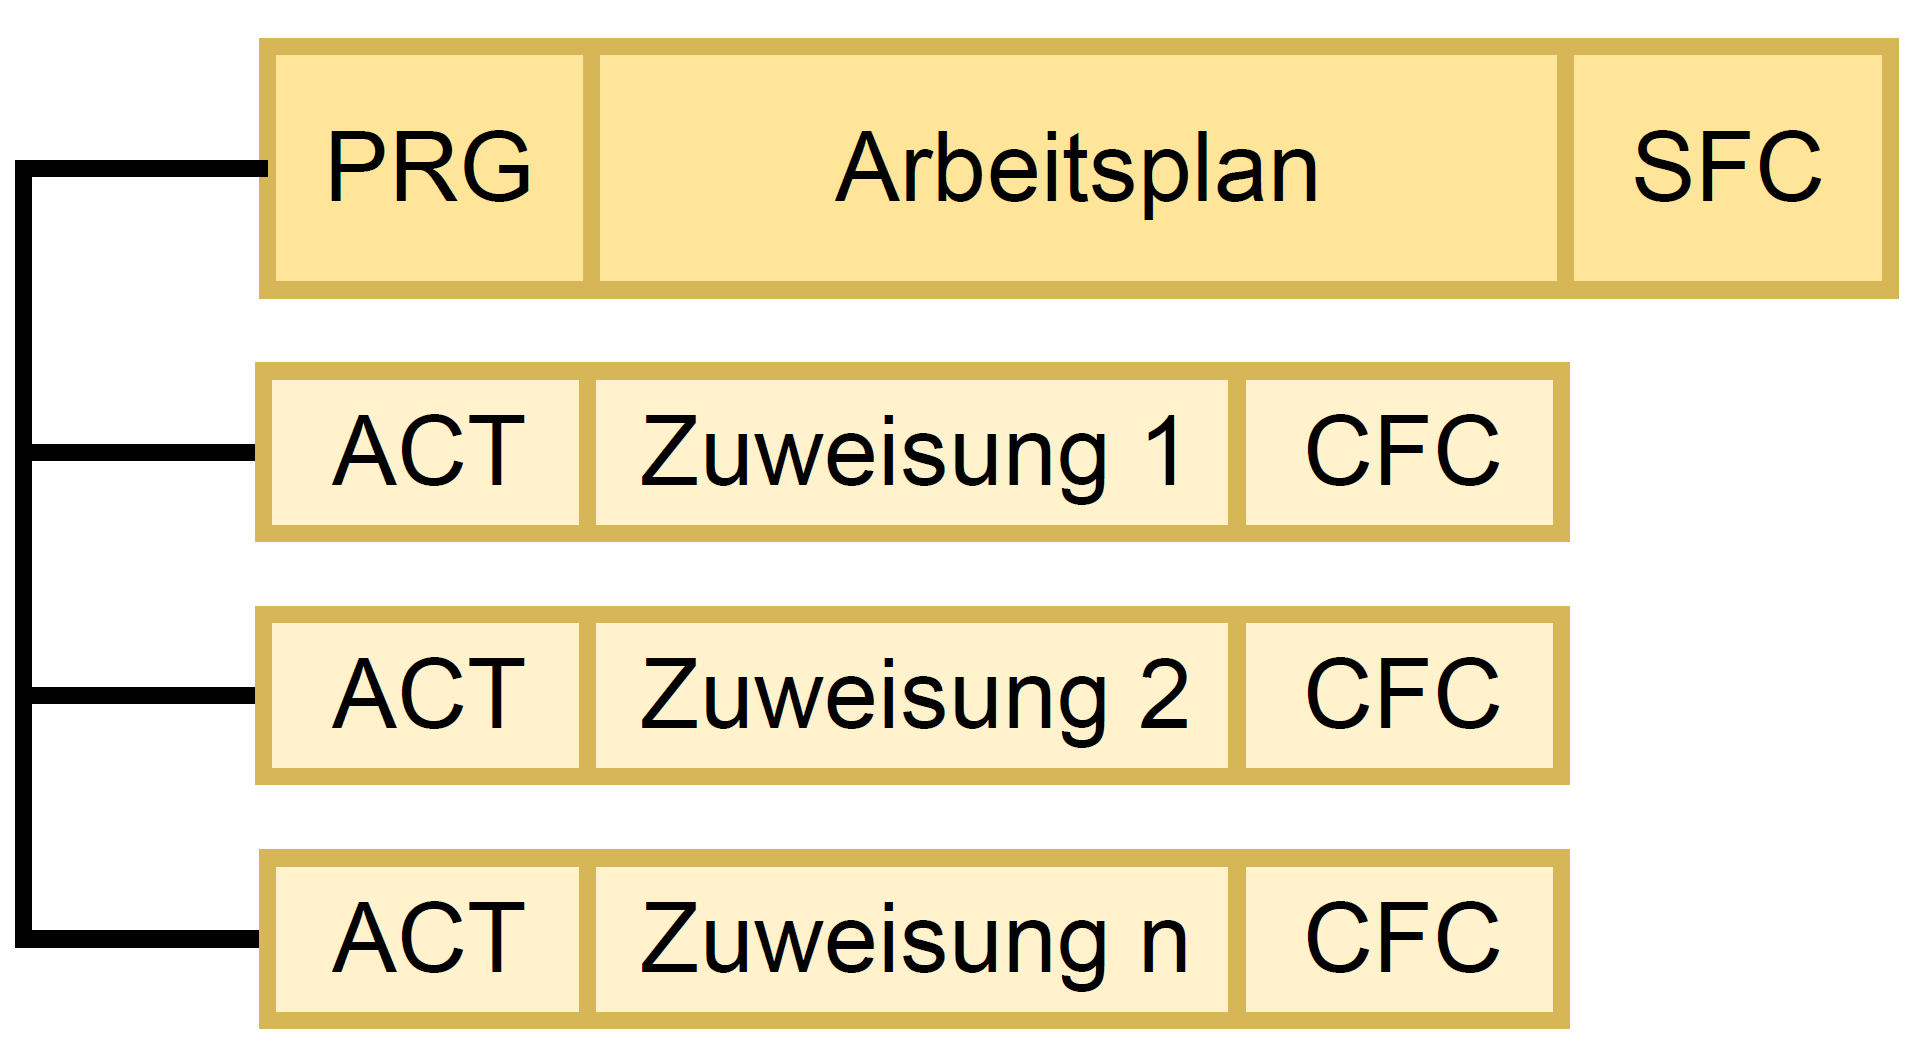
\includegraphics[width=0.5\textwidth]{08_Prozessmodell/Arbeitsplanaufbau}
			\captionsetup{justification=centering}
			\caption{Aufbau eines Arbeitsplans}
			\label{fig:Arbeitsplanaufbau}
		\end{figure}
		
		Bei der Variablendeklaration des Arbeitsplanes werden folgende Elemente instanziiert: 
		
		\begin{itemize}
			\item Bedienparameter
			\item Prozessparameter
			\item Skill-Instanzen
			\item Sequenz-Instanzen
		\end{itemize}
		\vspace{2mm}
		Die Bedienparameter dienen zum Start des Ablaufs. Unter Prozessparameter werden alle Parameter zusammengefasst, die für den Betrieb des Arbeitsplans erforderlich sind. Alle Informationen, die als Eingabevariablen für Skills und Sequenzen verwendet werden, müssen in diesem Bereich definiert sein. Die Instanzen von Skills und Sequenzen repräsentieren die im Arbeitsplan verwendeten Skills und Sequenzen.
		\\
		Die Prozessparameter könnten über eine «Rezeptverwaltung» verwaltet werden. Damit bietet TwinCAT die Möglichkeit benutzerdefinierte Variablenlisten zu erstellen und zu verwalten. Für einen Arbeitsplan könnte dadurch einfach ein bestimmtes Rezept geladen werden, welches sämtliche Prozessvariablen enthält. Dieses Feature wurde innerhalb dieser Arbeit noch nicht implementiert. 
		
			